% Build here: pdflatex -interaction=nonstopmode -halt-on-error report.tex (twice).
% Figures are clipped directly from the supplied paper at the repository root.
\pdfminorversion=5
\pdfobjcompresslevel=0
\documentclass[10pt,twocolumn]{article}
\usepackage[letterpaper,margin=0.68in,columnsep=0.25in]{geometry}
\usepackage[T1]{fontenc}
\usepackage{mathptmx,microtype,amsmath,booktabs,graphicx,caption,titlesec,flushend,needspace}
\usepackage[hidelinks]{hyperref}
\titleformat{\section}{\normalsize\bfseries}{\thesection.}{0.45em}{}
\titlespacing*{\section}{0pt}{8pt}{4pt}
\captionsetup{font=small,labelfont=bf,skip=4pt}
\setlength{\parindent}{1em}
\setlength{\parskip}{1pt}
\setlength{\textfloatsep}{10pt}
\setlength{\intextsep}{9pt}
\raggedbottom
\newcommand{\lookup}{\textsc{Lookup}}
\newcommand{\expand}{\textsc{Expand}}
\newcommand{\code}[1]{{\small\texttt{#1}}}
\begin{document}
\twocolumn[\begin{center}
{\LARGE\bfseries Diamond-Hardened Hash Joins in PostgreSQL\par}
\vspace{5pt}
{\normalsize CS631 Midterm Report: Executor Implementation and Microbenchmark\par}
\vspace{6pt}
{\small
\begin{tabular}{@{}c@{\hspace{1.3em}}c@{\hspace{1.3em}}c@{\hspace{1.3em}}c@{}}
Harshit Raj & Sumedh SS & Kabir S Prakash & Harshul Suthar\\
23B0950 & 23B1079 & 23B1036 & 23B0968
\end{tabular}\par}
\vspace{7pt}
\end{center}]

\noindent\textbf{Abstract.}
A sequence of binary joins can generate millions of intermediate tuples even
when its input relations and final result are small. We implement the
Lookup--Expand decomposition of Birler et al.~[1] in PostgreSQL's executor.
Lookup checks whether a match exists and saves its hash-table position; Expand
generates the matches only after subsequent lookups have removed unsuccessful
partial tuples. The implementation preserves duplicate rows and keeps saved
positions valid until expansion. On a deterministic three-relation acyclic
microbenchmark, the native-to-Diamond speedups are 200.99$\times$ at
$N=1{,}000$ and 669.27$\times$ at $N=5{,}000$. This report focuses on the execution
mechanism and microbenchmark; automatic cost-based plan selection and broader
evaluation are reserved for subsequent work.

\section{Problem and applicable queries}
A binary hash join builds a hash table on one input and probes it with the
other. Each probe produces every matching pair. If a later join rejects most
of those pairs, the database has already spent time generating, evaluating,
and passing a large intermediate result. Figure~\ref{fig:diamond} illustrates
this \emph{diamond problem}: the amount of data grows and then shrinks.
The intermediate need not be stored in full; generating it in a pipeline is
already expensive.

\begin{figure}[ht]
\centering
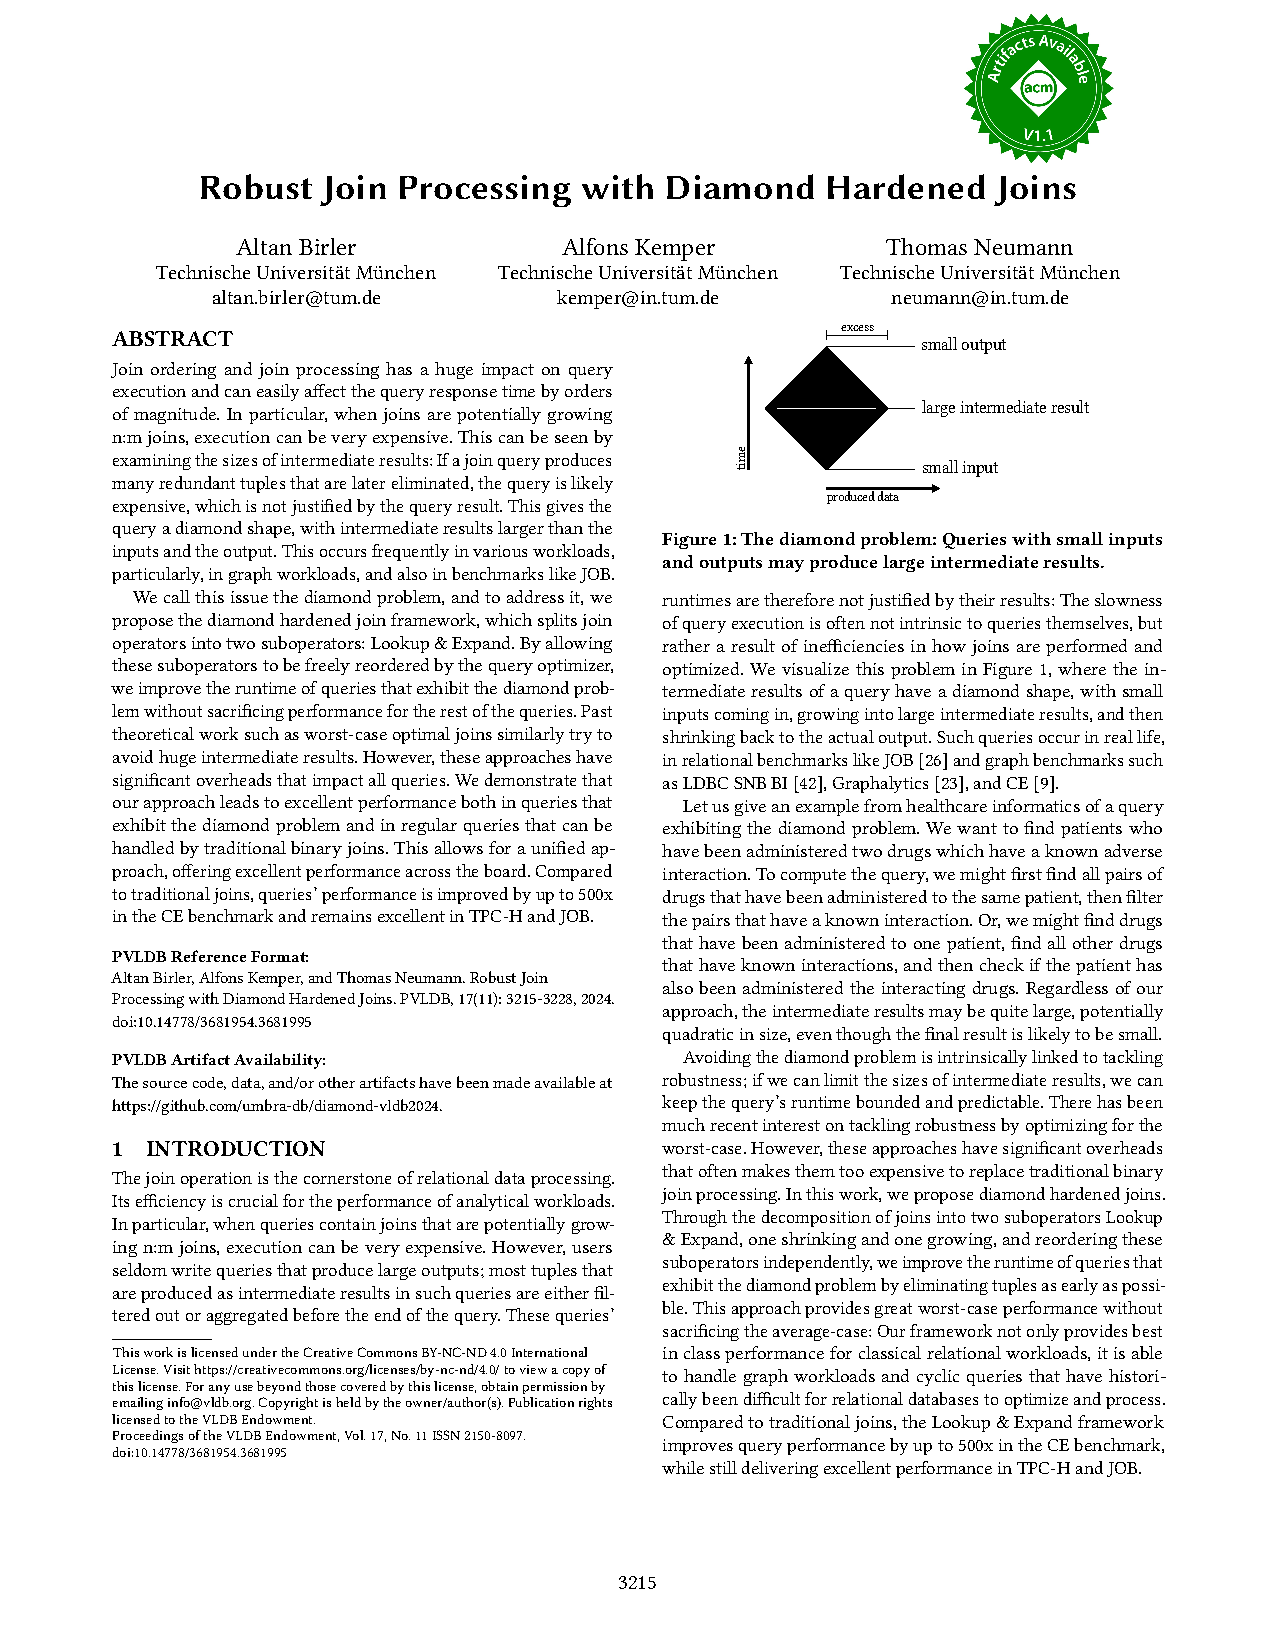
\includegraphics[page=1,trim=340bp 540bp 69bp 154bp,clip,width=.88\columnwidth]{../../../p3215-birler.pdf}
\caption{Small input and output can conceal a large intermediate.
Reproduced from [1], Figure~1.}
\label{fig:diamond}
\end{figure}

The opportunity arises in \textbf{chains}, such as
$X(a,b)\bowtie Y(b,c)\bowtie Z(c,d)$, when fanout on one edge is rejected by
another; in \textbf{stars}, where a central tuple is checked against several
relations; and in longer \textbf{acyclic trees}, where a distant relation
eliminates otherwise productive matches. These shapes alone do not guarantee
a speedup. The relevant combination is many matches followed by substantial
rejection. A primary-key lookup with at most one match has little expansion
to avoid, while a genuinely large final output must still be enumerated.

For intuition, consider patients joined with administered drugs and a relation
of interacting drug pairs: most generated pairs may fail the final interaction
check. Such application patterns motivate the paper's broader treatment,
including cyclic predicates. Our demonstrated scope here is single-process
inner hash equijoins whose retained hash tables remain in memory.

\section{The paper's Lookup--Expand idea}
The paper separates the two tasks hidden inside a hash probe.
\textbf{Lookup} finds the first equality match. If none exists, it discards
the input tuple. Otherwise it returns one \emph{head}, the paper's term for
the current partial result tuple together with a saved position for matches
that have not yet been generated.
\textbf{Expand} uses that saved position to emit each matching joined tuple.
Adjacent Lookup and Expand reproduce an ordinary inner hash join, including
all duplicates; merely renaming the operations offers no algorithmic gain.

The gain comes from moving an independent Lookup before an Expand.
In Figure~\ref{fig:rewrite}, $R_1(a,b)$ can probe $R_2(a)$ and $R_3(b)$
using keys already present in that partial tuple. The rightmost plan checks both
relations before enumerating either result. If the second check fails, it
rejects that tuple and implicitly all matches saved by the first check.
The circled arrow denotes Lookup and the circled \emph{e} denotes Expand;
dashed links connect deferred data to its later expansion.

\begin{figure}[ht]
\centering
\includegraphics[page=5,trim=317bp 107bp 39bp 585bp,clip,width=\columnwidth]{../../../p3215-birler.pdf}
\caption{Binary joins (left), decomposition (middle), and Lookup
pushdown (right). Reproduced from [1], Figure~3.}
\label{fig:rewrite}
\end{figure}

This reordering is legal only when the next lookup key is available in the
partial tuple: columns from a deferred match become available only after
expansion. In an $\alpha$-acyclic join, GYO can repeatedly remove a relation
whose shared join attributes are contained in one remaining parent relation.
The removal order gives the Lookups, and reversing it gives the Expands. Saved
match positions travel with partial tuples through larger trees. Cyclic joins
require additional machinery such as the paper's ternary Expand3, outside this
report's implementation scope.

\section{PostgreSQL execution}
PostgreSQL uses demand-pull execution: each plan node returns one tuple whenever
its parent asks for the next one. A normal Hash Join first reads one input and
builds a hash table. For every tuple from the other input, it computes the join
key, finds the corresponding bucket, and returns matching tuples one at a time.
Across repeated requests, it drains that bucket while the parent tests and may
reject each joined tuple separately. Thus a high-fanout probe still generates
a large stream even when almost every tuple is later rejected.

\Needspace{5\baselineskip}
Our implementation represents Lookup and Expand as separate executor nodes.
Lookup uses PostgreSQL's existing hash table and equality checks, but stops
after finding the first real match. It saves the input tuple and its current
position in the bucket, then returns the surviving partial tuple. This lets
another Lookup test it before any remaining matches are generated. Expand later
returns the saved first match and resumes the same bucket position until it is
exhausted. Each call to Expand returns one joined tuple and saves its position.
When the parent asks for another tuple, Expand advances to the next matching
hash-table entry. A saved tuple with $k$ matches therefore returns all $k$
rows, including duplicates, over $k$ successful calls.

One $N=5{,}000$ \code{EXPLAIN ANALYZE} run is summarized below. The
complete PostgreSQL output is shown in the demonstration:
\begin{quote}\footnotesize\ttfamily\raggedright
Native: X--Y intermediate = 24,985,001 rows\\
Native: final = 1 row; time = 2146.301 ms\\[2pt]
Diamond Lookup: Y against Z hash = 4,999 candidates\\
Hash the surviving Y candidates on b\\
Diamond Lookup: X against Y hash = 1 candidate\\
Two Expands: final = 1 row; fallback = false\\
Diamond time = 3.101 ms
\end{quote}
The native lower join sends 24,985,001 tuples to its parent before one survives.
Diamond's first Lookup sends 4,999 candidate tuples to the next check; it leaves
one, so both Expands are asked to produce only the single surviving result.

No new index is required. Lookup reuses PostgreSQL's hash tables, while the
saved positions remain private executor state. EXPLAIN shows Lookup and Expand
as plan nodes; unsupported cases use PostgreSQL's ordinary plan. Execution is
single-process, and each retained hash table must remain in one in-memory batch
so that its saved positions stay valid until Expand runs.

\section{Microbenchmark: why expansion is wasted}
We use a deterministic instance of $X(a,b)$, $Y(b,c)$, and $Z(c,d)$:
\begin{align*}
X &= \{(1,1)\}\cup\{(i,2):1\leq i\leq N\},\\
Y &= \{(1,1)\}\cup\{(2,c):4\leq c\leq N\}\\
  &\quad\cup\{(b,3):3\leq b\leq N\},\\
Z &= \{(1,1)\}\cup\{(3,i):1\leq i\leq N\}.
\end{align*}
Both $X$ and $Z$ contain $N+1$ rows; $Y$ contains $2N-4$ rows.
The query returns every matching tuple, without aggregation:
\begin{quote}\small\ttfamily
SELECT x.a, x.b, y.c, z.d\\
FROM X x JOIN Y y ON x.b = y.b\\
JOIN Z z ON y.c = z.c;
\end{quote}

Joining $X$ and $Y$ first produces $N(N-3)+1$ rows: $N$ rows with
$b=2$ each match $N-3$ rows of $Y$. None of these matches has a
$c$ present in $Z$. Starting with $Y\bowtie Z$ also grows to $N(N-2)+1$
rows, whose $b\geq3$ values are absent from $X$. Thus simply reversing the
two binary joins does not remove the problem. Only $(1,1,1,1)$ survives
all predicates.

The recorded Diamond plan first builds a hash table on $Z.c$ and scans $Y$.
Lookup retains $N-1$ candidate $Y$ tuples: the special tuple and the $N-2$
tuples with $c=3$. PostgreSQL then builds an intermediate hash table on their
$b$ values, storing each $Y$ tuple with its saved position in the $Z$ table.
It scans $X$ and probes this table. Since $X$ contains only $b=1$ and $b=2$,
all candidates with $b\geq3$ are rejected. Only the special tuple reaches the
two Expands, yielding one row. At $N=5{,}000$, the first Lookup carries 4,999
candidates and the second leaves one, avoiding the native plan's 24,985,001
intermediate pairs. For this family of inputs, the dominant work changes
from quadratic intermediate generation to linear hash build and probe work.

\section{Results}
Table~\ref{tab:results} shows the measured execution times. For
$N=1{,}000$ and $N=5{,}000$, native PostgreSQL and Diamond returned exactly
the same rows, including duplicates. Each time is the median of three
\code{EXPLAIN ANALYZE} runs. The Diamond plan uses two Lookups followed by
two Expands and completes without falling back to the native plan.

\begin{table}[ht]
\centering\small
\setlength{\tabcolsep}{4pt}
\begin{tabular}{rrrr}\toprule
$N$ & Native (ms) & Diamond (ms) & Speedup\\\midrule
1,000 & 212.040 & 1.055 & 200.99$\times$\\
5,000 & 2,625.554 & 3.923 & 669.27$\times$\\
50,000 & timeout & 30.785 & --\\\bottomrule
\end{tabular}
\caption{Median execution times. Native exceeded 120 seconds at
$N=50{,}000$, so no speedup is reported for that size.}
\label{tab:results}
\end{table}

At $N=50{,}000$, native PostgreSQL did not finish within 120 seconds,
so only the Diamond time is shown. This benchmark deliberately creates a
large intermediate result, so the same speedup should not be expected for
every query. Although the hash tables fit in memory, native PostgreSQL still
spends quadratic CPU work generating intermediate rows.

\section{Scope and next steps}
The midterm establishes the executor mechanism and its benefit on the
acyclic microbenchmark. Subsequent work will calibrate automatic plan selection
and use JOB and TPC-H to assess coverage and end-to-end gains. The central
result here is specific: delaying expansion allows later joins to reject whole
groups of matches before PostgreSQL pays to enumerate them.

\vspace{4pt}
\noindent\small\textbf{Reference}\par
\noindent\small [1] A. Birler, A. Kemper, and T. Neumann.
\emph{Robust Join Processing with Diamond Hardened Joins}.
PVLDB 17(11):3215--3228, 2024. doi:10.14778/3681954.3681995.
Figures reproduced from the supplied paper (CC BY-NC-ND 4.0).
\end{document}
